\documentclass{article}[11pt]


%\documentclass[runningheads,a4paper]{llncs}
%\usepackage{hyperref}
%\usepackage{ amssymb }


%\gasset{frame=false} % switch to true to add frames
%\parindent=0pt

%\usepackage{bussproofs}
%\usepackage{varwidth}
%\usepackage{xspace}
%\usepackage{verbatim}


\usepackage[lmargin=4cm, rmargin=4cm, tmargin=3cm, bmargin=3cm]{geometry}
\usepackage{algpseudocode}


\usepackage{url}
\usepackage{multirow} 
\usepackage{mathtools}
\usepackage{stmaryrd}
\DeclarePairedDelimiter{\ceil}{\lceil}{\rceil}
\DeclarePairedDelimiter{\floor}{\lfloor}{\rfloor} 
%\usepackage{xspace}
\usepackage{latexsym,amsmath,amsfonts,amssymb,stmaryrd}
\let\proof\relax
\let\endproof\relax 
\usepackage{amsthm} 
\usepackage{tikz}
\usepackage{tikz-qtree}
\usepackage{tikz-qtree-compat}

\usepackage{listings}
\usepackage{chngpage}
\DeclareMathAlphabet{\mathpzc}{OT1}{pzc}{m}{it}

\usepackage{ amssymb }
\usepackage{soul}

\usepackage{tipa}
\usepackage{stmaryrd}

\usepackage{verbatim} 
\usepackage{epsfig} 
\usepackage{graphics}
\usepackage{ mathrsfs }
\usepackage{hyperref}
\usepackage{multicol}

\usepackage{epigraph}


% \usepackage{tipa}
\usepackage{graphicx}   
%\usepackage{url}
\usepackage{wrapfig}  
\usepackage{bm}   
\usepackage{epstopdf}  
\usepackage{ upgreek }
\usepackage[all,cmtip]{xy}

\usepackage{natbib}
% \usepackage{float} 
% \usepackage[lofdepth,lotdepth]{subfig}
%\usepackage{graphicx}
\usepackage[T1]{fontenc} 
\usepackage[utf8]{inputenc}
\usepackage{etoolbox}
\usepackage{textcomp}

\usepackage{mdwtab}
\usepackage{syntax} 

\renewcommand{\syntleft}{}          % do not display '<' associated with variable, for example <A>
\renewcommand{\syntright}{}         % do not display '>' associated with variable, for example <A>


\makeatletter 
\patchcmd{\maketitle}{\@copyrightspace}{}{}{}
\makeatother 
\usepackage{mathpartir}
%\usepackage{enumitem}

%\usepackage{supertabular} 
%\usepackage{soul}
\usepackage[all]{xy}
\usepackage{xifthen}
\usepackage{placeins} 
\usepackage{amsthm}
\usepackage{amsmath}


\usepackage{pgf}
\usepackage{tikz}
\usetikzlibrary{arrows,automata}
\tikzset{initial text={}}
\usetikzlibrary{calc,shapes.multipart,chains,arrows}
%prevents second paragraph indentations 
%\usepackage{parskip}
% \usepackage{floatrow}
\usepackage{tabularx} % in the preamble
\usepackage{bm}
\usepackage{caption}
\usepackage{subcaption} 

%\input{mac}s

\newtheorem{theorem}{Theorem}
\newtheorem{lemma}[theorem]{Lemma}


\title{Bases formelles du TAL  \\ DM sur les $\epsilon$-transitions }

\author{Pierre-Léo Bégay}
\date{À me rendre le 6 mars 2020}
\theoremstyle{definition}
\newtheorem{exmp}{Exemple}
   

\begin{document}
 
\maketitle
\pagestyle{empty} %
\thispagestyle{empty}

\newpage
%% Attention: pas plus d'un recto-verso!
% Ne conservez pas les questions

\section{$\epsilon$-transitions}

\subsection{Définitions}

On donne parfois la définition suivante d'un AFND : 


\[
A =  \big \langle Q,\Sigma,q_0,F,\delta \big \rangle
\]

\begin{itemize}
\item[] $Q$ ensemble fini d'états
\item[] $\Sigma$ l'alphabet (ensemble de lettres)
\item[] $q_0$ l'état initial
\item[] $F \subseteq Q$, les états terminaux
\item[] $\delta$ fonction de $(Q \times (\Sigma \cup \{\epsilon\}))$ dans $2^Q$ 
\end{itemize}

Par rapport à la définition du cours, on revient à un seul état initial et qu'on permet d'étiqueter des transitions par $\epsilon$. Ces transitions, appelées $\epsilon$-transitions, sont \textit{gratuites}, par contraste avec les transitions normales qui \textit{consomment} une lettre chaque fois qu'on les emprunte. La notion d'acceptation est sinon la même que pour les AFND qu'on a déjà vus. 

\subsection{Exemples}



\begin{figure}[!h]
\centering

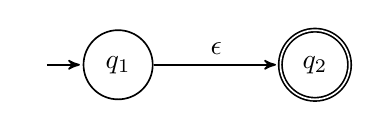
\begin{tikzpicture}[->,>=stealth',shorten >=1pt,auto,node distance=2.5cm,
                    semithick]
  \tikzstyle{every state}=[fill=white,text=black]
  \tikzstyle{place}=[rectangle,draw=black,fill=white, minimum size=7mm]


  \node[initial, state] (S)                    {$q_1$};
  \node[state,accepting] (A)      [right of=S]                {$q_2$};

  \path (S) edge      []        node {$\epsilon$} (A);
\end{tikzpicture}
\caption{Automate $A_1$}
\end{figure}

Dans l'automate $A_1$, aucune transition par lettre n'est possible, ce qui empêche d'accepter tout mot autre que le mot vide. Ce dernier est cependant reconnu car on peut emprunter \textit{gratuitement} l'unique transition et atterrir dans un état terminal.


\begin{figure}[!h]
\centering

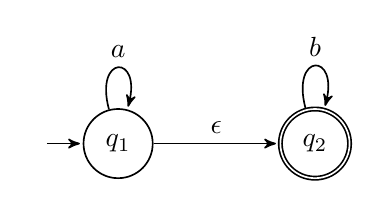
\begin{tikzpicture}[->,>=stealth',shorten >=1pt,auto,node distance=2.5cm,
                    semithick]
  \tikzstyle{every state}=[fill=white,text=black]
  \tikzstyle{place}=[rectangle,draw=black,fill=white, minimum size=7mm]


  \node[initial, state] (S)                    {$q_1$};
  \node[state,accepting] (A)      [right of=S]                {$q_2$};

  \path (S) edge[loop above]              node {$a$} (S)
(S) edge      []        node {$\epsilon$} (A)
 (A) edge[loop above]              node {$b$} (A);
\end{tikzpicture}
\caption{Automate $A_2$}
\end{figure}
\newpage
L'automate $A_2$ reconnait quant à lui le langage $a^*b^*$. En effet, on peut boucler avec des $a$ sur $q_1$ puis, une fois qu'on a fini, on passe gratuitement à $q_2$ (sans consommer de $a$ ou de $b$) où on peut boucler avec des $b$ jusqu'à avoir fini le mot.

\begin{figure}[!ht]
\centering

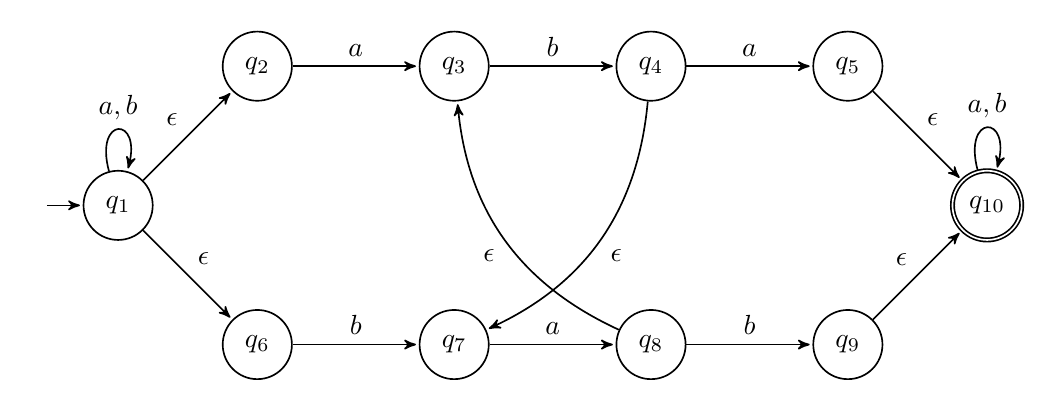
\begin{tikzpicture}[->,>=stealth',shorten >=1pt,auto,node distance=2.5cm,
                    semithick]
  \tikzstyle{every state}=[fill=white,text=black]
  \tikzstyle{place}=[rectangle,draw=black,fill=white, minimum size=7mm]


  \node[initial, state] (S)                    {$q_1$};
  \node[state] (A)      [above right of=S]                {$q_2$};
  \node[state] (B)      [right of=A]                {$q_3$};
  \node[state] (C)      [right of=B]                {$q_4$};
    \node[state] (D)      [right of=C]                {$q_5$};
  \node[state] (E)      [below right of=S]                {$q_6$};
  \node[state] (F)      [right of=E]                {$q_7$};
    \node[state] (G)      [right of=F]                {$q_8$};    \node[state] (H)      [right of=G]                {$q_9$};
        \node[state,accepting] (I)      [above right of=H]                {$q_{10}$};
  
  \path (S) edge[loop above]              node {$a,b$} (S)
 (I) edge[loop above]              node {$a,b$} (I)
(S) edge      []        node {$\epsilon$} (A)
(A) edge      []        node {$a$} (B)
(B) edge      []        node {$b$} (C)
(C) edge      []        node {$a$} (D)
(D) edge      []        node {$\epsilon$} (I)
(S) edge      []        node {$\epsilon$} (E)
(E) edge      []        node {$b$} (F)
(F) edge      []        node {$a$} (G)
(G) edge      []        node {$b$} (H)
(H) edge      []        node {$\epsilon$} (I)
(C) edge      [bend left]        node {$\epsilon$} (F)
(G) edge      [bend left]        node {$\epsilon$} (B);
\end{tikzpicture}
\caption{Automate $A_3$}
\end{figure}

Enfin, l'automate $A_3$, proche d'un qu'on a vu en cours, reconnaît quant à lui le langage $\Sigma^*aba\Sigma^* + \Sigma^*bab\Sigma^*$ (les deux $\epsilon$-transitions en croix ne permettent pas d'accepter plus de mots).



\section{Lecture d'automates avec $\epsilon$-transitions}


Décrivez les langages reconnus par les automates $A_4$, $A_5$ et $A_6$ à l'aide d'une expression rationelle. Essayez de justifier, au moins informellement, votre réponse. 

\begin{figure}[!h]
\centering

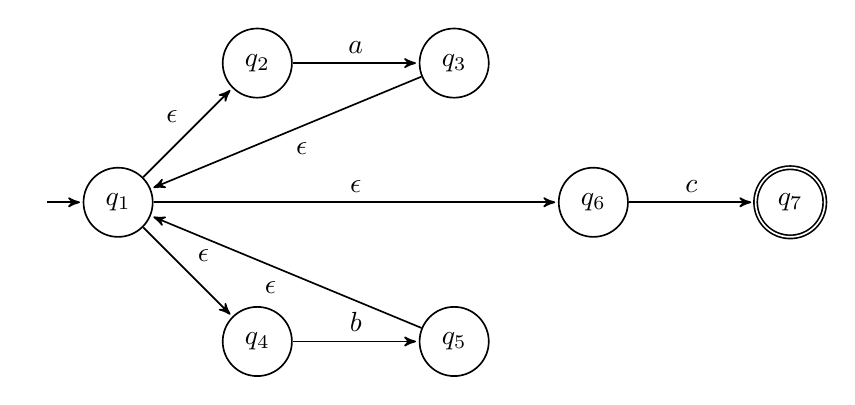
\begin{tikzpicture}[->,>=stealth',shorten >=1pt,auto,node distance=2.5cm,
                    semithick]
  \tikzstyle{every state}=[fill=white,text=black]
  \tikzstyle{place}=[rectangle,draw=black,fill=white, minimum size=7mm]


  \node[initial, state] (S)                    {$q_1$};
  \node[state] (A)      [above right of=S]                {$q_2$};
  \node[state] (B)      [right of=A]                {$q_3$};
  \node[state] (C)      [below right of=S]                {$q_4$};
    \node[state] (D)      [right of=C]                {$q_5$};
  \node[state] (E)      [above right of=D]                {$q_6$};
  \node[state,accepting] (F)      [right of=E]                {$q_7$};
    
  
  \path %(I) edge[loop above]              node {$a,b$} (I)
(S) edge      []        node {$\epsilon$} (A)
(A) edge      []        node {$a$} (B)
(B) edge      []        node {$\epsilon$} (S)
(S) edge      []        node {$\epsilon$} (C)
(C) edge      []        node {$b$} (D)
(D) edge      []        node {$\epsilon$} (S)
(S) edge      []        node {$\epsilon$} (E)
(E) edge      []        node {$c$} (F);
\end{tikzpicture}
\caption{Automate $A_4$}
\end{figure}



\begin{figure}[!h]
\centering

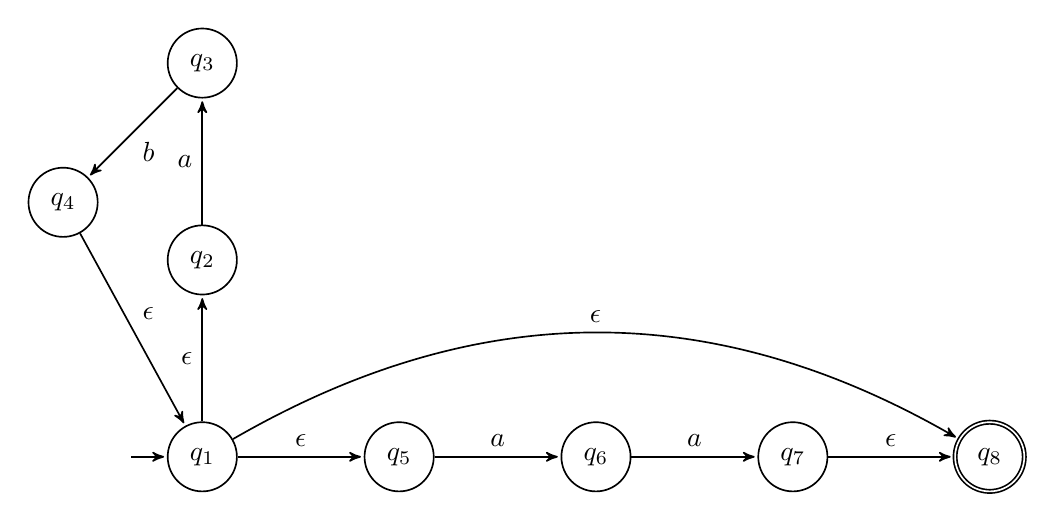
\begin{tikzpicture}[->,>=stealth',shorten >=1pt,auto,node distance=2.5cm,
                    semithick]
  \tikzstyle{every state}=[fill=white,text=black]
  \tikzstyle{place}=[rectangle,draw=black,fill=white, minimum size=7mm]


  \node[initial, state] (S)                    {$q_1$};
  \node[state] (A)      [above of=S]                {$q_2$};
  \node[state] (B)      [above of=A]                {$q_3$};
  \node[state] (C)      [below left of=B]                {$q_4$};
    \node[state] (D)      [right of=S]                {$q_5$};
  \node[state] (E)      [right of=D]                {$q_6$};
  \node[state] (F)      [right of=E]                {$q_7$};
    \node[state,accepting] (G)      [right of=F]                {$q_8$};    
    
  
  \path %(I) edge[loop above]              node {$a,b$} (I)
(S) edge      []        node {$\epsilon$} (A)
(A) edge      []        node {$a$} (B)
(B) edge      []        node {$b$} (C)
(C) edge      []        node {$\epsilon$} (S)
(S) edge      []        node {$\epsilon$} (D)
(D) edge      []        node {$a$} (E)
(E) edge      []        node {$a$} (F)
(F) edge      []        node {$\epsilon$} (G)
(S) edge      [bend left]        node {$\epsilon$} (G);
\end{tikzpicture}
\caption{Automate $A_5$}
\end{figure}

\newpage

\begin{figure}[!h]
\centering
 
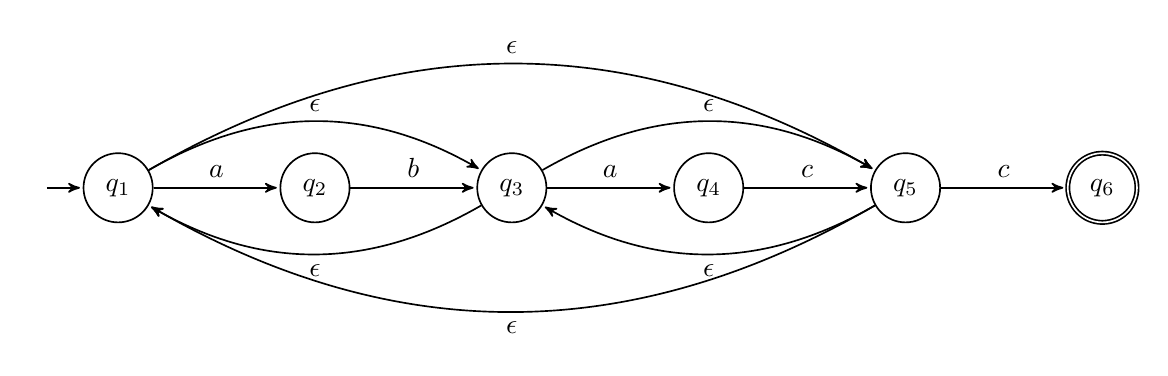
\begin{tikzpicture}[->,>=stealth',shorten >=1pt,auto,node distance=2.5cm,
                    semithick]
  \tikzstyle{every state}=[fill=white,text=black]
  \tikzstyle{place}=[rectangle,draw=black,fill=white, minimum size=7mm]


  \node[initial, state] (S)                    {$q_1$};
  \node[state] (A)      [right of=S]                {$q_2$};
  \node[state] (B)      [right of=A]                {$q_3$};
  \node[state] (C)      [right of=B]                {$q_4$};
    \node[state] (D)      [right of=C]                {$q_5$};
  \node[state,accepting] (E)      [right of=D]                {$q_6$};

    
  
  \path %(I) edge[loop above]              node {$a,b$} (I)
(S) edge      []        node {$a$} (A)
(A) edge      []        node {$b$} (B)
(S) edge      [bend left]        node {$\epsilon$} (B)
(B) edge      [bend left]        node {$\epsilon$} (S)
(B) edge      [bend left]        node {$\epsilon$} (D)
(D) edge      [bend left]        node {$\epsilon$} (B)
(S) edge      [bend left]        node {$\epsilon$} (D)
(D) edge      [bend left]        node {$\epsilon$} (S)
(B) edge      []        node {$a$} (C)
(C) edge      []        node {$c$} (D)
(D) edge      []        node {$c$} (E);
\end{tikzpicture}
\caption{Automate $A_6$}
\end{figure}


\paragraph*{Correction} Dans $A_4$, le cycle $q_1 \xrightarrow{\epsilon} q_2 \xrightarrow{a} q_3 \xrightarrow{\epsilon} q_1$ permet de boucler sur l'état initial $q_1$ en lisant un $a$. De même, le cycle $q_1 \xrightarrow{\epsilon} q_4 \xrightarrow{b} q_5 \xrightarrow{\epsilon} q_1$ permet lui de boucler en lisant un b. On peut donc lire autant de $a$ et de $b$ qu'on veut au début du mot. Ensuite, le segment $q_1 \xrightarrow{\epsilon} q_6 \xrightarrow{c} q_7$ amène à l'état terminal en lisant un c. Une fois arrivé, on ne peut plus rien lire. Le langage reconnu est donc $(a+b)^*c$

\paragraph*{} Dans $A_5$, le circuit $q_1 \xrightarrow{\epsilon} q_2 \xrightarrow{a} q_3 \xrightarrow{b} q_4 \xrightarrow{\epsilon} q_1$ permet de boucler sur $q_1$ en lisant $ab$. Une fois qu'on a fini de boucler, on peut soit lire $aa$ en parcourant $q_1 \xrightarrow{\epsilon} q_5 \xrightarrow{a} q_6 \xrightarrow{a} q_7 \xrightarrow{\epsilon} q_8$, soit aller directement de $q_1$ à $q_8$ avec une $\epsilon$-transition. Une fois arrivé, on ne peut plus rien lire. Le langage reconnu est donc $(ab)^*((aa)+\epsilon)$

\paragraph*{}Dans $A_6$, on peut utiliser les $\epsilon$-transitions pour circuler librement entre $q_1$, $q_3$ et $q_5$ (notez que les transitions entre $q_1$ et $q_5$ sont inutiles). Via $q_1 \xrightarrow{a} q_2 \xrightarrow{b} q_3$ on lit $ab$, et $q_3 \xrightarrow{a} q_4 \xrightarrow{c} q_5$ nous fait lire $ac$. On peut donc lire autant de fois $ab$ et $ac$ qu'on veut, avant de lire un $c$ en faisant $q_5 \xrightarrow{c} q_6$, où on ne peut plus rien faire. Le langage reconnu est donc $((ab)+(ac))^*c$.


\section{Elimination d'$\epsilon$-transitions}

On propose une méthode pour éliminer les $\epsilon$-transitions s'appuyant sur la fonction $\epsilon^+$ de type $Q \rightarrow 2^Q$ définie de la façon suivante :

\begin{figure}[!h]
\begin{enumerate}
\item Si $q_j \in \delta(q_i,\epsilon)$, alors $q_j \in \epsilon^+(q_i)$
\item Si $q_j \in \epsilon^+(q_i)$ et $q_k \in \delta(q_j,\epsilon)$, alors $q_k \in \epsilon^+(q_i)$
\end{enumerate}
\caption{Définition de $\epsilon^+$}
\label{eplusdef}
\end{figure}
 
 
A partir d'un automate non-déterministe avec $\epsilon$-transitions  $\big \langle Q,\Sigma,q_0,F,\delta \big \rangle$, on génère un automate non-déterministe équivalent sans $\epsilon$-transitions  $\big \langle Q,\Sigma,q_0,F',\delta' \big \rangle$ avec l'algorithme suivant :

\begin{figure}[!h]
\begin{algorithmic}[1]
\State $F' := F$
\ForAll {$q_i \in Q$}
    \ForAll {$c \in \Sigma$}
        $\delta'(q_i,c) := \delta(q_i,c)$
    \EndFor
\EndFor
\ForAll{$q_i \in Q$ tels que $\epsilon^+(q_i) \neq \emptyset$}
	\ForAll{$q_j \in \epsilon^+(q_i)$}
		\ForAll{$c \in \Sigma$ et $q_r \in Q$ tels que $q_r \in \delta(q_j,c)$}
			\State $\delta'(q_i,c) := \delta'(q_i,c) \cup \{q_r\}$
		\EndFor
		\If {$q_j \in F$}
			\State $F' := F' \cup \{q_i\}$
		\EndIf
	\EndFor
\EndFor
\end{algorithmic}
\caption{Algorithme d'élimination des $\epsilon$-transitions}
\label{algo}
\end{figure}
\vspace{2cm}
\paragraph*{Question 1} Pour chaque automate ($A_1$ à $A_6$), calculez la fonction $\epsilon^+$ en vous servant de la définition en figure \ref{eplusdef}. Vous devriez donner l'image de chaque état, par exemple $\epsilon^+(q_1) = \{q_1,q_2\}$, $\epsilon^+(q_2) = \emptyset$ etc. 

\paragraph{Remarque} On corrige en même temps les questions 1 et 2.

\paragraph*{Question 2} Pour chaque automate ($A_1$ à $A_6$), appliquez l'algorithme de la figure \ref{algo}. Vous pouvez dessiner le résultat. Pas besoin de détailler tous les calculs. 


\paragraph*{Correction pour $A_1$} 
\begin{itemize}
\item[] $\epsilon^+(q_1) = \{\textcolor{red}{q_2}\}$\footnote{En \textcolor{red}{rouge} on note les états terminaux, pour appliquer la règle des lignes 11/12 de l'algorithme.}
\item[] $\epsilon^+(q_2) = \emptyset$
\end{itemize}


\begin{figure}[!h]
\centering

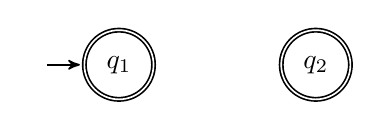
\begin{tikzpicture}[->,>=stealth',shorten >=1pt,auto,node distance=2.5cm,
                    semithick]
  \tikzstyle{every state}=[fill=white,text=black]
  \tikzstyle{place}=[rectangle,draw=black,fill=white, minimum size=7mm]


  \node[initial, state,accepting] (S)                    {$q_1$};
  \node[state,accepting] (A)      [right of=S]                {$q_2$};

\end{tikzpicture}
\caption{Automate $A_1'$}
\end{figure}

\paragraph*{}Notez que l'état $q_2$ est devenu inaccessible. Techniquement il fait toujours partie de l'automate (l'ensemble d'états n'est pas modifié par l'algorithme), mais on pourrait bien sûr raisonnablement le `jeter`.


\paragraph*{Correction pour $A_2$} 
\begin{itemize}
\item[] $\epsilon^+(q_1) = \{\textcolor{red}{q_2}\}$
\item[] $\epsilon^+(q_2) = \emptyset$
\end{itemize}


\begin{figure}[!h]
\centering

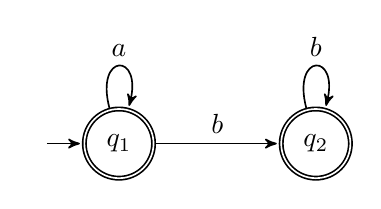
\begin{tikzpicture}[->,>=stealth',shorten >=1pt,auto,node distance=2.5cm,
                    semithick]
  \tikzstyle{every state}=[fill=white,text=black]
  \tikzstyle{place}=[rectangle,draw=black,fill=white, minimum size=7mm]


  \node[initial,accepting, state] (S)                    {$q_1$};
  \node[state,accepting] (A)      [right of=S]                {$q_2$};

  \path (S) edge[loop above]              node {$a$} (S)
(S) edge      []        node {$b$} (A)
 (A) edge[loop above]              node {$b$} (A);
\end{tikzpicture}
\caption{Automate $A_2'$}
\end{figure}


\paragraph*{Correction pour $A_3$} 
\begin{itemize}
\item[] $\epsilon^+(q_1) = \{q_2,q_6\}$
\item[] $\epsilon^+(q_2) = \emptyset$
\item[] $\epsilon^+(q_3) = \{\}$
\item[] $\epsilon^+(q_4) = \{q_7\}$
\item[] $\epsilon^+(q_5) = \{\textcolor{red}{q_{10}}\}$
\item[] $\epsilon^+(q_6) = \emptyset$
\item[] $\epsilon^+(q_7) = \emptyset$
\item[] $\epsilon^+(q_8) = \{q_3\}$
\item[] $\epsilon^+(q_9) = \{\textcolor{red}{q_{10}}\}$
\item[] $\epsilon^+(q_{10}) = \emptyset$
\end{itemize}


\begin{figure}[!h]
\centering

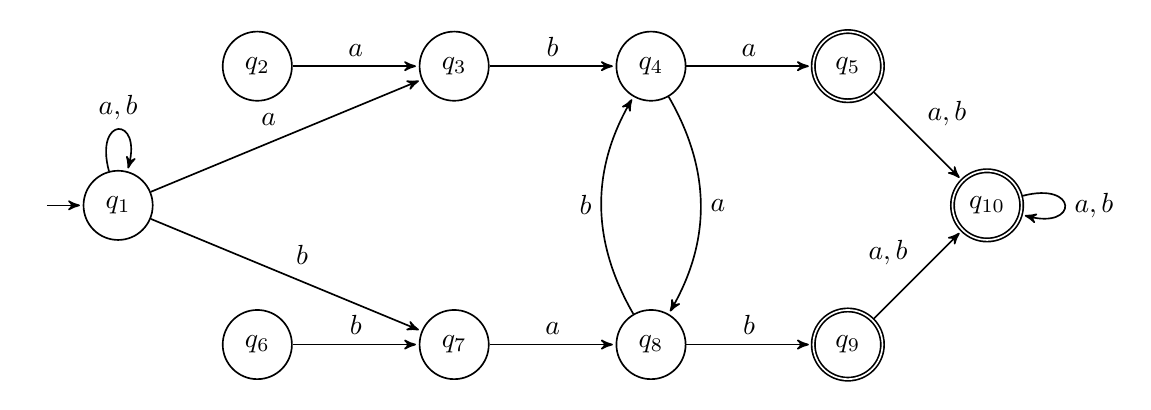
\begin{tikzpicture}[->,>=stealth',shorten >=1pt,auto,node distance=2.5cm,
                    semithick]
  \tikzstyle{every state}=[fill=white,text=black]
  \tikzstyle{place}=[rectangle,draw=black,fill=white, minimum size=7mm]


  \node[initial, state] (S)                    {$q_1$};
  \node[state] (A)      [above right of=S]                {$q_2$};
  \node[state] (B)      [right of=A]                {$q_3$};
  \node[state] (C)      [right of=B]                {$q_4$};
    \node[state,accepting] (D)      [right of=C]                {$q_5$};
  \node[state] (E)      [below right of=S]                {$q_6$};
  \node[state] (F)      [right of=E]                {$q_7$};
    \node[state] (G)      [right of=F]                {$q_8$};    \node[state,accepting] (H)      [right of=G]                {$q_9$};
        \node[state,accepting] (I)      [above right of=H]                {$q_{10}$};
  
  \path (S) edge[loop above]              node {$a,b$} (S)
 (I) edge[loop right]              node {$a,b$} (I)
(S) edge      []        node {$a$} (B)
(A) edge      []        node {$a$} (B)
(B) edge      []        node {$b$} (C)
(C) edge      []        node {$a$} (D)
(D) edge      []        node {$a,b$} (I)
(S) edge      []        node {$b$} (F)
(E) edge      []        node {$b$} (F)
(F) edge      []        node {$a$} (G)
(G) edge      []        node {$b$} (H)
(H) edge      []        node {$a,b$} (I)
(C) edge      [bend left]        node {$a$} (G)
(G) edge      [bend left]        node {$b$} (C);
\end{tikzpicture}
\caption{Automate $A_3'$}
\end{figure}

\paragraph*{}Notez que l'automate $A_3'$ n'est ni minimal, ni déterministe (t qu'il y a encre des états inaccessibles).



\paragraph*{Correction pour $A_4$} 
\begin{itemize}
\item[] $\epsilon^+(q_1) = \{q_2,q_4,q_6\}$
\item[] $\epsilon^+(q_2) = \emptyset$
\item[] $\epsilon^+(q_3) = \{q_1,q_2,q_4,q_6\}$
\item[] $\epsilon^+(q_4) = \emptyset$
\item[] $\epsilon^+(q_5) = \{q_1,q_2,q_4,q_6\}$
\item[] $\epsilon^+(q_6) = \emptyset$
\end{itemize}


% (a+b)*(c)
\begin{figure}[!h]
\centering

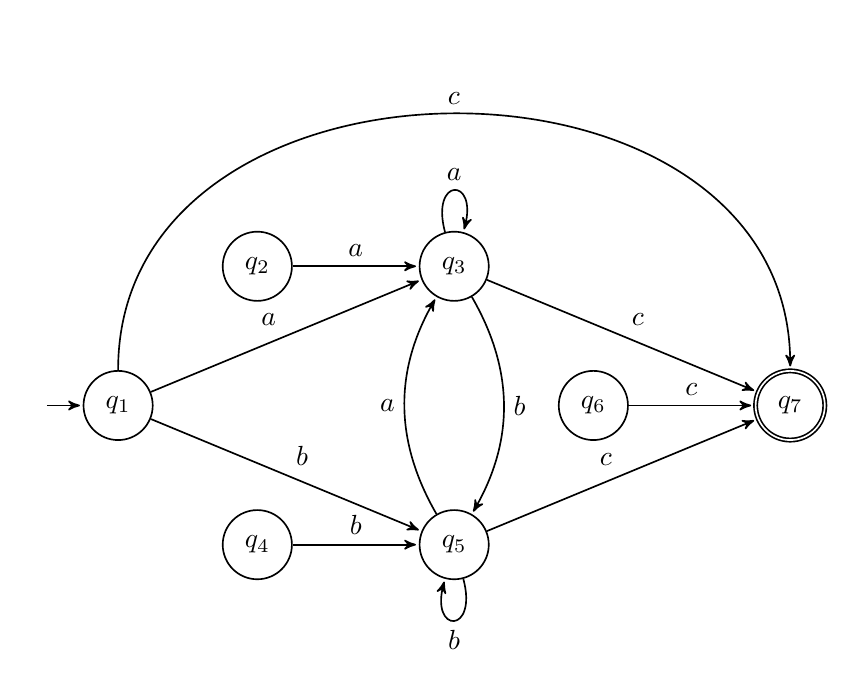
\begin{tikzpicture}[->,>=stealth',shorten >=1pt,auto,node distance=2.5cm,
                    semithick]
  \tikzstyle{every state}=[fill=white,text=black]
  \tikzstyle{place}=[rectangle,draw=black,fill=white, minimum size=7mm]


  \node[initial, state] (S)                    {$q_1$};
  \node[state] (A)      [above right of=S]                {$q_2$};
  \node[state] (B)      [right of=A]                {$q_3$};
  \node[state] (C)      [below right of=S]                {$q_4$};
    \node[state] (D)      [right of=C]                {$q_5$};
  \node[state] (E)      [above right of=D]                {$q_6$};
  \node[state,accepting] (F)      [right of=E]                {$q_7$};
    
  
  \path %(I) edge[loop above]              node {$a,b$} (I)
(S) edge      []        node {$a$} (B)
(A) edge      []        node {$a$} (B)
(B) edge      []        node {$c$} (F)
(B) edge      [bend left]        node {$b$} (D)
(B) edge      [loop above]        node {$a$} (B)
(D) edge      [loop below]        node {$b$} (D)
(S) edge      []        node {$b$} (D)
(S) edge      [bend left=90, looseness=1.3]        node {$c$} (F)
(C) edge      []        node {$b$} (D)
(D) edge      [bend left]        node {$a$} (B)
(D) edge      []        node {$c$} (F)
(E) edge      []        node {$c$} (F);
\end{tikzpicture}
\caption{Automate $A_4'$}
\end{figure}

\paragraph*{Correction pour $A_5$} 
\begin{itemize}
\item[] $\epsilon^+(q_1) = \{q_2,q_5,\textcolor{red}{q_8}\}$
\item[] $\epsilon^+(q_2) = \emptyset$
\item[] $\epsilon^+(q_3) = \emptyset$
\item[] $\epsilon^+(q_4) = \{q_1,q_2,q_5,\textcolor{red}{q_8}\}$
\item[] $\epsilon^+(q_5) = \emptyset$
\item[] $\epsilon^+(q_6) = \emptyset$
\item[] $\epsilon^+(q_7) = \{\textcolor{red}{q_8}\}$
\item[] $\epsilon^+(q_9) = \emptyset$
\end{itemize}


\begin{figure}[!h]
\centering

\begin{tikzpicture}[->,>=stealth',shorten >=1pt,auto,node distance=2.5cm,
                    semithick]
  \tikzstyle{every state}=[fill=white,text=black]
  \tikzstyle{place}=[rectangle,draw=black,fill=white, minimum size=7mm]


  \node[initial, state, accepting] (S)                    {$q_1$};
  \node[state] (A)      [above of=S]                {$q_2$};
  \node[state] (B)      [above of=A]                {$q_3$};
  \node[state,accepting] (C)      [below left of=B]                {$q_4$};
    \node[state] (D)      [right of=S]                {$q_5$};
  \node[state] (E)      [right of=D]                {$q_6$};
  \node[state,accepting] (F)      [right of=E]                {$q_7$};
    \node[state,accepting] (G)      [right of=F]                {$q_8$};    
    
  
  \path %(I) edge[loop above]              node {$a,b$} (I)
(S) edge      [bend right]        node {$a$} (B)
(S) edge      [bend right]        node {$a$} (E)
(A) edge      []        node {$a$} (B)
(B) edge      []        node {$b$} (C)
(C) edge      [bend left]        node {$a$} (B)
(C) edge      [bend right=90, looseness=1.5]        node {$a$} (E)
(D) edge      []        node {$a$} (E)
(E) edge      []        node {$a$} (F);
\end{tikzpicture}
\caption{Automate $A_5'$}
\end{figure}


\paragraph*{Correction pour $A_6$} 
\begin{itemize}
\item[] $\epsilon^+(q_1) = \{q_1,q_3,q_5\}$
\item[] $\epsilon^+(q_2) = \emptyset$
\item[] $\epsilon^+(q_3) = \{q_1,q_3,q_5\}$
\item[] $\epsilon^+(q_4) = \emptyset$
\item[] $\epsilon^+(q_5) = \{q_1,q_3,q_5\}$
\item[] $\epsilon^+(q_6) = \emptyset$
\end{itemize}


\begin{figure}[!h]
\centering

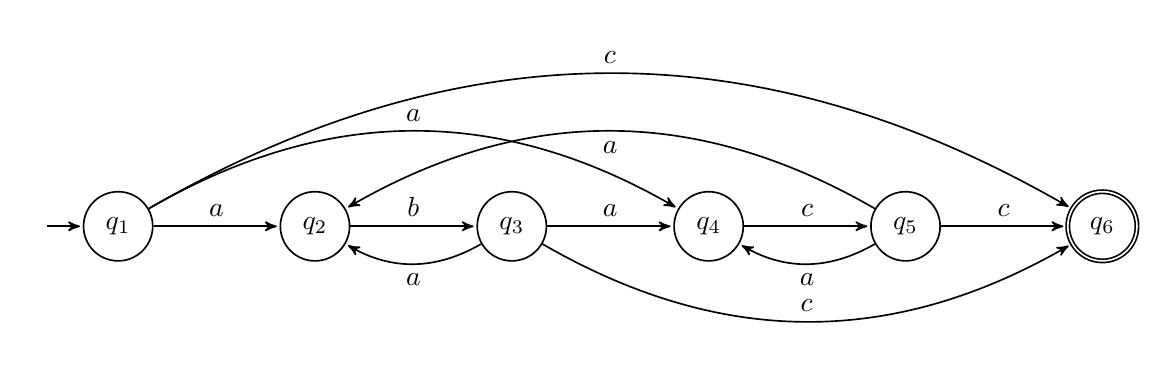
\begin{tikzpicture}[->,>=stealth',shorten >=1pt,auto,node distance=2.5cm,
                    semithick]
  \tikzstyle{every state}=[fill=white,text=black]
  \tikzstyle{place}=[rectangle,draw=black,fill=white, minimum size=7mm]


  \node[initial, state] (S)                    {$q_1$};
  \node[state] (A)      [right of=S]                {$q_2$};
  \node[state] (B)      [right of=A]                {$q_3$};
  \node[state] (C)      [right of=B]                {$q_4$};
    \node[state] (D)      [right of=C]                {$q_5$};
  \node[state,accepting] (E)      [right of=D]                {$q_6$};

    
  
  \path %(I) edge[loop above]              node {$a,b$} (I)
(S) edge      []        node {$a$} (A)
(A) edge      []        node {$b$} (B)
(S) edge      [bend left]        node {$c$} (E)
(S) edge      [bend left]        node {$a$} (C)
(B) edge      [bend left]        node {$a$} (A)
(B) edge      [bend right]        node {$c$} (E)
(D) edge      [bend left]        node {$a$} (C)
(D) edge      [bend right]        node {$a$} (A)
(B) edge      []        node {$a$} (C)
(C) edge      []        node {$c$} (D)
(D) edge      []        node {$c$} (E);
\end{tikzpicture}
\caption{Automate $A_6'$}
\end{figure}



\paragraph*{Question 3} Essayez d'expliquer en français la fonction $\epsilon^+$ et l'algorithme comme si vous vouliez me convaincre qu'ils font correctement leur boulot (ce qui est le cas)\footnote{Notez que rien n'est gratuit dans l'algorithme et que chaque \textit{morceau} a un sens. Vous devriez donc tout mentionner.}. Vous pouvez vous aider d'exemples, soit tirés de la question précédente, soit originaux.


\paragraph*{Correction} La fonction $\epsilon^+$ associe à chaque état $q_i$ l'ensemble des états qui sont accessible par une $\epsilon$-transition (règle 1 de la fonction) ou plusieurs (la \textbf{récursion} de la règle 2). Par exemple, dans la correction de l'élimination des $\epsilon$-transitions de l'automate $A_5$, les états $q_2, q_5$ et $q_8$ sont intégrés à $e^+(q_4)$ par la deuxième règle de la définition de la fonction car on peut y accéder depuis $q_4$ en deux coups d'$\epsilon$

\paragraph*{}L'automate produit (ou renvoyé) par l'algorithme a le même ensemble d'états et le même initial que l'automate donné en entrée. Ce qui change, ce sont donc les transitions et les états terminaux.

\paragraph*{Les transitions} Déjà, la boucle des lignes 2 à 4 de l'algorithme permet de \textit{garder} dans le nouvel automate toutes les `non-$\epsilon$-transitions` données\footnote{Pour rappel, $\epsilon$ ne fait pas partie de $\Sigma$. Il est \textit{rajouté} à la liste des symboles pouvant étiqueter une transition dans la définition du $\delta$ d'un automate avec $\epsilon$-transitions}. Toute transition par $a$, $b$ etc dans l'automate original apparaîtra donc également dans la version sans $\epsilon$-transition. 

\paragraph*{}La seconde boucle s'intéresse à chaque triplet d'états $q_i$, $q_j$ et $q_r$ tels que $q_i \xrightarrow{\epsilon}^+ q_j \xrightarrow{c} q_r$, c'est à dire tels que $q_i$ peut atteindre $q_j$ avec une ou plusieurs $\epsilon$-transitions et $q_j$ va en $q_r$ avec une transition \textit{normale} avec $c$. 

\paragraph*{}Pour chacun de ces triplets $q_i \xrightarrow{\epsilon}^+ q_j \xrightarrow{c} q_r$, on ajoute (ligne 9) la transition $q_i \xrightarrow{c} q_r$. Le sens de cette règle est que quand, depuis un état, on peut \textit{se préparer} à une \textit{vraie} transition avec une série d'$\epsilon$-transitions, alors on peut la faire directement sans bouger au préalable. 

\paragraph*{Etats terminaux}De plus, si un état non-terminal peut atteindre un état terminal via des $\epsilon$-transitions, il accepte le mot vide. Il faut donc \textit{garder} ça même après l'élimination des transitions, d'où le fait qu'on ajoute ces états à $F'$ (lignes 11/12).

\paragraph*{Version plus technique} Soit le mot $w = c_1c_2...c_n$ accepté par l'automate avec $\epsilon$-transitions (appelé $A$). Il existe donc dans cet automate un chemin pour le mot en alternant \textit{vraies transitions} et (potentiellement) une ou plusieurs $\epsilon$-transitions. Le chemin est donc de la forme :\newline

$q_{u_1} \xrightarrow{\epsilon}^* q_{u_2} \xrightarrow{c_1} q_{u_3} \xrightarrow{\epsilon}^* q_{u_4} \xrightarrow{c_2} q_{u_5}~...~q_{u_{2n-2}} \xrightarrow{\epsilon}^* q_{u_{2n-1}} \xrightarrow{c_{n}} q_{u_{2n+1}} \xrightarrow{\epsilon}^* q_{u_{2n+2}} $ \newline

avec $q_{u_{2n+2}} \in F$.\newline

Pour rappel, chaque $q_{u_i} \xrightarrow{\epsilon}^* q_{u_{i+1}} \xrightarrow{c} q_{u_{i+2}}$ représente un passage de $q_{u_i}$ à $q_{u_{i+1}}$ avec aucune ou un nombre strictement positif d'$\epsilon$-transitions puis à $q_{u_{i+2}}$ en lisant $c$. \newline

Dans le premier cas, on a $q_{u_i} = q_{u_{i+1}}$ (puisqu'on n'a pas bougé), on peut donc enlever la (non-)transition du chemin et passer directement de $q_{u_i}$ à $q_{u_{i+2}}$ avec $c$. \newline

Dans le second cas, $q_{u_{i+1}} \in \epsilon^+(q_{u_i})$. On a donc ajouté la transition $q_{u_i} \xrightarrow{c} q_{u_{i+2}}$ à l'automate produit par l'automate ($A'$). \newline

Le chemin donné plus haut correspond donc, dans l'automate produit, à :\newline

$q_{u_1}~\textcolor{white}{\xrightarrow{\epsilon}^* q_{u_2}} \xrightarrow{c_1} q_{u_3} \textcolor{white}{\xrightarrow{\epsilon}^* q_{u_4}} \xrightarrow{c_2} q_{u_5}~...~q_{u_{2n-2}} \textcolor{white}{\xrightarrow{\epsilon}^* q_{u_{2n-1}}} ~\xrightarrow{c_{n}} q_{u_{2n+1}}$\newline

De plus, puisque $q_{u_{2n+1}} \in \epsilon^+(q_{2n+2})$, $q_{u_{i+1}}$ est un état terminal dans l'automate produit (s'il ne l'était pas déjà dans l'original). La lecture du mot s'arrête donc sur un état acceptant. Le mot $w$, qui était accepté dans l'automate initial, est donc également accepté dans l'automate produit par l'algorithme.

\paragraph*{}Pour faire les choses bien, il faudrait également montrer que l'algorithme n'ajoute pas des mots acceptés, c'est à dire qu'il n'existe pas de $w$ accepté par $A'$ et pas par $A$. La démonstration est un peu plus lourde que la précédente mais en utilisant un raisonnement par l'absurde on retrouve au fond le même principe.

\paragraph*{}En gros, on suppose qu'un tel mot existe. Il existe donc un chemin dans $A'$ qui accepte $w$. Si toutes les transitions du chemin étaient déjà présentes dans $A$ et que le dernier état était à l'origine terminal, alors l'exact même chemin aurait accepté $w$ dans $A$. Au moins une de deux propositions est donc fausse.

\paragraph*{}Si il est faux que toutes les transitions étaient déjà dans $A$, au moins une ne l'était pas. Or, si des transitions $q_i \xrightarrow{c} q_j$ apparaissent dans $A'$, c'est que $q_j$ était accessible depuis $q_i$ avec des $\epsilon$-transitions puis $c$. On peut donc `retrouver` toutes ces transitions dans $A$.

\paragraph*{}S'il est faux que le dernier état du chemin était terminal dans $A$, alors il l'est devenu. Or, la seule façon dont l'algorithme peut un état terminal est s'il peut atteindre un terminal avec une série d'$\epsilon$-transitions. On peut donc, dans $A$, rajouter des $\epsilon$-transitions au chemin pour atteindre un état terminal.

\paragraph*{}Tout chemin acceptant $w$ dans $A'$ peut donc être transformé en un chemin acceptant dans $A$ acceptant le même mot. L'algorithme n'ajoute donc pas de nouveaux mots.

\paragraph*{Conclusion} Tout mot accepté par $A$ est accepté par $A'$, et inversement. L'algorithme est donc conforme à sa spécification.



\section{Formalisation}

\paragraph*{Question 4} Donnez une formalisation de l'acceptation d'un mot dans le contexte des AFND avec $\epsilon$-transtion en adaptant la définition de $\delta^*$ donnée dans le cours.

\paragraph*{Correction} On adapte la formalisation des AFND vue en cours :
 
\begin{itemize}
\item $\delta^*(q,\epsilon$\footnote{Attention, il s'agit ici du mot vide, pas d'une $\epsilon$-transition !}$) = \{q\}$
\item $\delta^*(q,a.w) = \displaystyle\bigcup_{q' \in \{q\}~\cup~ \epsilon^+(q)}~\displaystyle\bigcup_{q'' \in \delta(q',a)} \delta^*(q'',w)$
\end{itemize}

\paragraph*{}La première disjonction $\bigcup$ permet d'utiliser des $\epsilon$-transitions pour passer de $q$ à un des états $q'$ accessibles gratuitement. La deuxième disjonction renvoie l'ensemble des états accessibles via une transition normale depuis l'état choisi.

\paragraph*{}Pour l'acceptation, on veut partir du seul état initial $i$, lire le mot donné et vérifier qu'on a atteint un état terminal ou qu'on peut en atteindre un gratuitement avec des $\epsilon$-transitions. On dit donc qu'un AFND avec $\epsilon$-transitions accepte un mot $w$ ssi. 

\[
\exists q_f \in ((\displaystyle\bigcup_{q~\in~\delta^*(i,w)} \{q\} \cup \epsilon^+(q)) \cap F)
\]


\paragraph*{Question bonus} Les AFND avec $\epsilon$-transitions sont-ils plus ou moins expressifs\footnote{cad. permettent-ils de décrire plus ou moins de langages ?} que ceux vus en cours, où on pouvait avoir plusieurs états initiaux ?

\paragraph*{Correction} Par rapport aux AFND du cours, les AFND avec $\epsilon$-transitions ont les $\epsilon$-transitions en plus et la possibilité d'avoir plusieurs états initiaux en moins. Puisqu'il existe un algorithme (justifié !) d'élimination des $\epsilon$-transitions qui produit un automate reconnaissant le même langage, l'utilisation d'$\epsilon$-transitions ne permet pas de reconnaître des langages que les AFND classiques ne peuvent pas représenter.

\paragraph*{}Il faut maintenant regarder si l'impossibilité d'avoir plusieurs états initiaux nous fait perdre de l'expressivité. Ce n'est pas le cas, parce que les $\epsilon$-transitions permettent de simuler la présence de plusieurs états initiaux. En effet, si on souhaite par exemple que les états $q_1$, $q_2$ et $q_3$ soient initiaux, il suffit d'ajouter un état $q_i$ initial, avec des $\epsilon$-transitions de $q_i$ vers les trois états sus-nommés.

\paragraph*{} Les changements entre AFND avec et sans $\epsilon$-transitions n'altèrent donc pas l'expressivité des modèles.

\paragraph*{Remarque} On aurait aussi pu contraindre les $AFND$ avec $\epsilon$-transitions en n'autorisant qu'un seul état terminal. En effet, soit un automate avec trois états terminaux $q_1$, $q_2$ et $q_3$, on pouvait les rendre "normaux" mais créer un unique état terminal $q_f$ avec des $\epsilon$-transitions de $q_1$, $q_2$ et $q_3$ vers $q_f$. En utilisant une astuce similaire, on aurait également pu obliger le déterminisme sur les transitions normales.

\paragraph*{Remarque bis} Puisque les $\epsilon$-transitions ne changent pas l'expressivité des AFND, on mélange en pratique les définitions, en autorisant plusieurs états initiaux, plusieurs transitions pour une même lettre et les $\epsilon$-transitions.  

\section{Propriétés de clôture}

\paragraph*{Question 5} Etant donnés des AFND (version $\epsilon$) représentant deux expressions rationnelles quelconques $e_1$ et $e_2$, expliquez, en vous aidant de schémas, comment construire des automates reconnaissant les expressions $e_1 + e_2$, $e_1.e_2$ et $e_1^*$.

\paragraph*{Question bonus} Répondre à la question précédente en utilisant la formalisation des automates.

\subsection{$e_1 + e_2$} On a $A_1$ et $A_2$ qui reconnaissent $e_1$ et $e_2$, respectivement. On a bien sûr envie de mettre les deux automates "l'un à côté de l'autre", mais on se retrouverait alors avec deux états initiaux. Soient $i_1$ et $i_2$ les états initiaux de $A_1$ et $A_2$, on les rend normaux et on ajoute un nouvel état $q_i$ initial, avec des $\epsilon$-transitions vers $i_1$ et $i_2$;

\paragraph*{Formalisation} Soient $A_1 = \big \langle Q_1,\Sigma_1,i_1,F_1,\delta_1 \big \rangle$ et $A_2 = \big \langle Q_2,\Sigma_2,i_2,F_2,\delta_2 \big \rangle$, on renvoie 

\[
\big \langle Q_1 \cup Q_2 \cup \{q_i\},\Sigma_1 \cup \Sigma_2,q_i,F_1 \cup F_2,\delta' \big \rangle
\]

où

\[
\begin{cases}
\delta'(q,a) = \delta_1(q,a) &\text{ si } q \in Q_1,\\[1ex]
\delta'(q,a) = \delta_2(q,a) &\text{ si } q \in Q_2,\\[1ex]
\delta'(q,\epsilon) = \delta_1(q,\epsilon) &\text{ si } q \in Q_1,\\[1ex]
\delta'(q,\epsilon) = \delta_2(q,\epsilon) &\text{ si } q \in Q_2,\\[1ex]
\delta'(q_i,\epsilon) = \{i_1,i_2\},\\[1ex]
\delta'(q_i,a) = \emptyset
 \end{cases}
\]


\subsection{$e_1.e_2$} On a $A_1$ et $A_2$ qui reconnaissent $e_1$ et $e_2$, respectivement. Le but est de faire une lecture dans $A_1$ puis une dans $A_2$. Pour ça, on met les automates à la suite l'un de l'autre, en ajoutant des $\epsilon$-transitions de chaque état terminal de $A_1$ vers l'état initial de $A_2$. Les états terminaux de $A_1$ ne le sont plus, tandis que l'état initial de $A_2$ devient également "normal".

\paragraph*{Formalisation} Soient $A_1 = \big \langle Q_1,\Sigma_1,i_1,F_1,\delta_1 \big \rangle$ et $A_2 = \big \langle Q_2,\Sigma_2,i_2,F_2,\delta_2 \big \rangle$, on renvoie 

\[
\big \langle Q_1 \cup Q_2 ,\Sigma_1 \cup \Sigma_2,i_1,F_2,\delta' \big \rangle
\]

où

\[
\begin{cases}
\delta'(q,a) = \delta_1(q,a) &\text{ si } q \in Q_1\\[1ex]
\delta'(q,a) = \delta_2(q,a) &\text{ si } q \in Q_2\\[1ex]
\delta'(q,\epsilon) = \delta_2(q,\epsilon) &\text{ si } q \in Q_2\\[1ex]
\delta'(q,\epsilon) = \delta_1(q,\epsilon) &\text{ si } q \in Q_1 \backslash F_1,\\[1ex]
\delta'(q,\epsilon) = \delta_1(q,\epsilon) \cup \{i_2\} &\text{ si } q \in Q_1 \cap F_1
 \end{cases}
\]



\subsection{$e_1^*$} On a $A_1$ qui reconnaît $e_1$. Le but est d'ajouter un état $S$ qui va permettre de faire des "tours de manège" dans $A_1$. $S$ est donc initial, et terminal (car $e_1^*$ accepte forcément le mot vide), a une $\epsilon$-transition vers l'état anciennement initial et en  reçoit une depuis tout état anciennement terminal (cf. le polycopié pour plus de détails).

\paragraph*{Formalisation} Soit $A_1 = \big \langle Q_1,\Sigma_1,i_1,F_1,\delta_1 \big \rangle$, on renvoie 

\[
\big \langle Q_1 \cup \{S\} ,\Sigma_1,S,\{S\},\delta' \big \rangle
\]

où

\[
\begin{cases}
\delta'(q,a) = \delta_1(q,a) &\\[1ex]

\delta'(q,\epsilon) = \delta_1(q,\epsilon) &\text{ si } q \in Q_1 \backslash F_1,\\[1ex]
\delta'(q,\epsilon) = \delta_1(q,\epsilon) \cup \{S\} &\text{ si } q \in Q_1 \cap F_1,\\[1ex]
\delta'(S,\epsilon) = \{i_1\}&\\[1ex]
\delta'(S,a) = \emptyset&
 \end{cases}
\]


\end{document} 
  


 
